\chapter{Analysis}

\section{Quality of time representation}

    Throughout this text, we use "decodability" as a proxy for quality of time representation. That is: we predict elapsed time from the neural activity, and the correctness of predictions measures how much information about time is contained in the activity. 

    \begin{figure}[ht!]
        \centering
        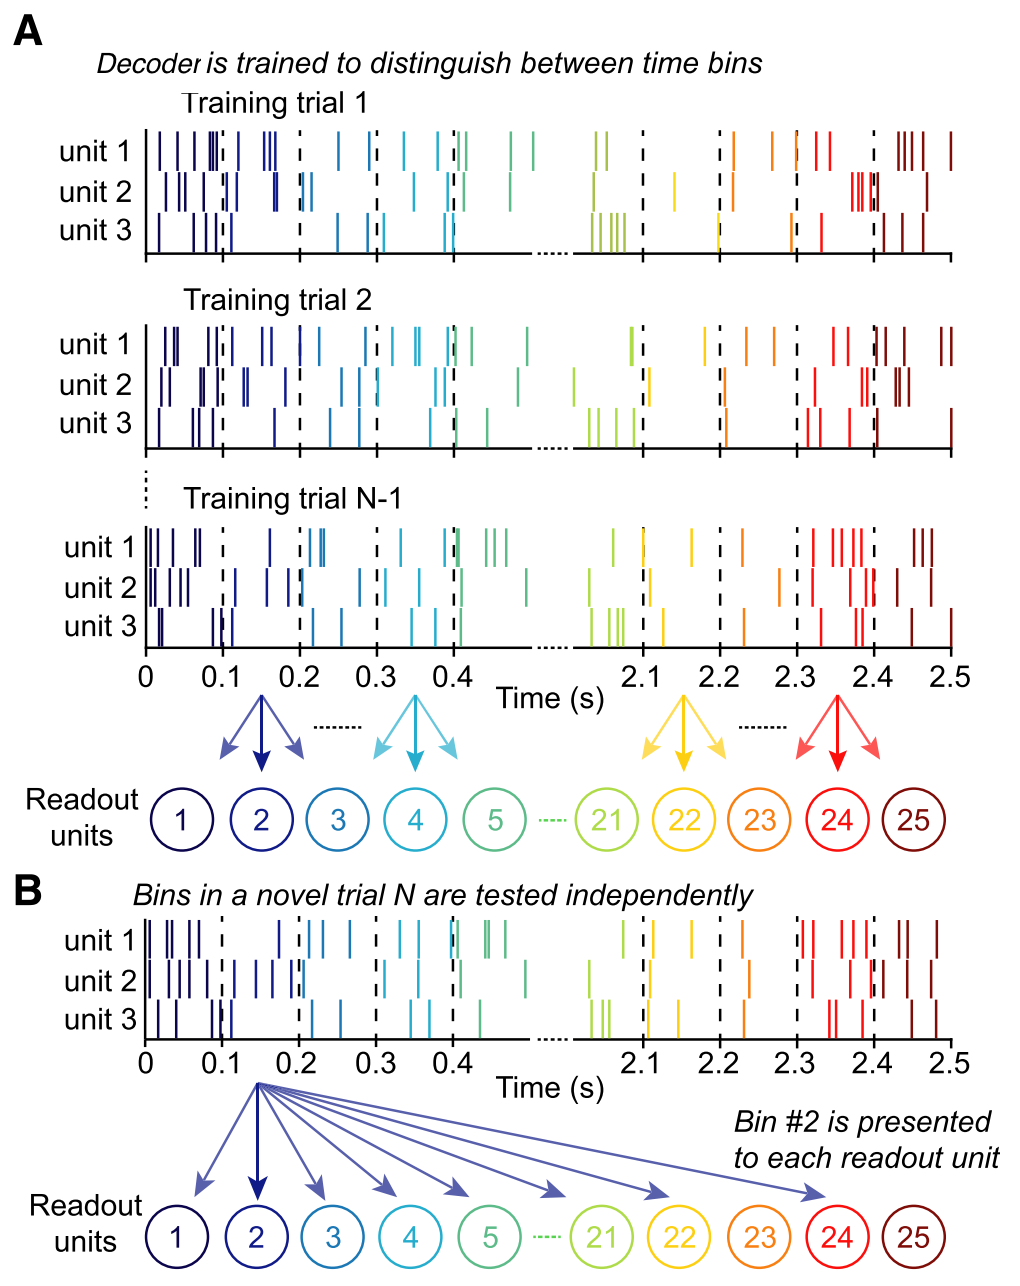
\includegraphics[width=0.83\textwidth]{figures/sketches/decoder.png}
        \caption[Classifier training sketch]{A, Training a classifier. Population activity for simultaneously recorded neurons (only 3 units represented) is transformed into firing rate estimates. The rate estimates are binned into 100 ms time bins. The classifier is trained to distinguish the population activity pattern in each time bin from every other time bin. The output can be illustrated by readouts of the probability per target time bin. B, The  model performance is evaluated using a Monte Carlo cross-validation approach, in which activity patterns from trials not used to train the model is presented to trained models. The example shows bin \#2 of some test trial. Modified from Bakhurin et al. \cite{bakhurin2017differential}}
        \label{fig:decoding}
    \end{figure}

    For each trial, the spike activity within the nosepoke was first transformed in a measure of population firing rate, following the steps described in Subsection \ref{subsec:fr_estimation}. Thereby, we obtained one population firing rate vector in 100~ms time bins, with each neuron corresponding to a vector coordinate. In the case of trials longer than 1.5s, only the first 15 bins were used for decoding analysis. 

    Elapsed time was then decoded from the population firing rates by either classification or regression. Classification requires a population vector to be strictly labeled as only one of the time bins, as illustrated in figure \ref{fig:decoding}. In turn, regression treats the decoding output as a continuous function, and therefore can provide intermediate values within a time bin, such as 450ms or 770ms.

    %Elapsed time was decoded from the population firing rates by either classification or regression. While classification requires a population vector to be labeled as one of the time bins, regression treats the output as a continuous function, and can give values such as 450ms or 770ms.
    Classification was implemented using Linear Discriminant Analysis (LDA) while regression used Bayesian Ridge. While many other algorithms were tested and corresponding hyperparameters tuned, we've chosen to advance our analysis using simpler and untuned algorithms. 

\section{Algorithm comparison}
    In the comparison between possible decoders, to find good hyperparameters for each, we applied a bayesian search using the scikit-optimization library \cite{skopt}. This procedure begins by randomly searching the parameter space, and after some iterations it starts to make estimates of the function values in the parameter space, sampling points with high estimated value. The fit of hyperparameter space is done by gausian processes, and its implementation is dealt with entirely by the library. The length of search was defined for each classifier depending on the number of hyperparameters to tune.
    
    We calculate the value at each point as the mean performance across a 5-fold cross-validation. All the procedure was done using a subset of half the data, selected as every other trial.
    
    We optimized classifiers for the pearson's r metric, and regressors for the explained variance (see section \ref{sec:metrics}).
    
    
    
\section{Bin shuffling}
    
    To test whether the methods used here were statistically significant, we randomized the data to produce ``surrogate'' datasets that, at the same time preserve global statistics and eliminate all causal effects. Applying the same method to the shuffled data, we can establish a baseline for the method and establish the chances of having significant effects by chance, and hence, measure the significance of the effects. The method we used here was the 
    bin shuffling and it was based on methods from \citeauthor{bakhurin2017differential} \cite{bakhurin2017differential}. It was used to break the temporal order of population activity, in such a way as to provide a null hypothesis for the neural activity prediction. To create the shuffled activity, each time bin in a trial was assigned a random activity vector from that trial, without replacement. In the end, each population activity vector is randomly assigned to a time point that does not relate to the original time point where the activity was extracted from.

\section{Performance metrics}
\label{sec:metrics}
    The metrics used for assessing model performance depended only on 1) the final output of the model (prediction) and 2) the correct time (tag). These metrics were given as follows:
    The prediction for all examples is the vector $\hat{y}$, while the correct tag for all the examples is the vector $y$. $N$ is the dimensionality of the vectors. $\bar{x}$ is the sample average of a variable $\sum_{i=1}^N{\frac{x_i}{N}}$. $\sigma$ is the unbiased standard deviation, and $\sigma^2$ is the unbiased variance, $\sigma^2(x) = \sum_{i=1}^N{\frac{(x_i - \bar x)^2}{N - 1}}$.

    % Nome em negrito pode ser suficiente
    \subsection{Explained variance}
        Explained variance provides a quantitative measure of how much the inclusion of the model can account for reducing the data variability. The computation of this measure contrasts the amount of variance in the residuals of the fitted model with the amount of variance in the original data.

        $$ \text{explained variance}(y, \hat{y}) = 1 - \frac{\sigma^2(y - \hat{y})}{\sigma^2(y)}$$
    
    \subsection{Pearson's r}
        Pearson's r is a measure of linear correlation, calculated by normalizing the linear covariance of two variables by their respective variances. 
        
        $$
        \text{Pearson's r}(y, \hat{y}) = 
        \frac{1}{n-1}\frac{\sum{(y - \bar{y})(\hat{y} - \bar{\hat{y}})}}
             {\sigma(y)\sigma{(\hat{y})}}
        $$
    
    \subsection{Modified accuracy}
        We modified the accuracy metric to enable its use in regression. Generally, accuracy is ill-defined for continuous targets, since it has no "similar enough" threshold. Our modified accuracy consists of rounding the continuous output to its closest value before measuring accuracy in its conventional sense. The notation $[\hat{y}]_y$ is the nearest value in $y$ for each value in $\hat{y}$. $\delta(x_1, x_2)$ is the Kronecker's delta, taking the value $1$ when $x_1 = x_2$ and $0$ otherwise. 
        
        $$
        \text{accuracy}(y, \hat{y}) = \frac{1}{N}\sum_{i=1}^{N}{\delta(y_i, [\hat{y}_i]_y)}
        $$
        
        
        
        
        